\documentclass[a4paper, 12pt, titlepage]{article}
\usepackage[utf8]{inputenc}
\usepackage[T1]{fontenc}
\usepackage[magyar]{babel}
\usepackage{graphicx}
\usepackage{siunitx}

\begin{document}

\begin{titlepage} %címoldal
\thispagestyle{empty}
\title{Feszültségtenzor, kontinuumok mozgásegyenlete \\és\\Általános Hook törvény, izotrop közegek rugalmas tulajdonságai\thanks{Folytonos közegek mechanikája gyakorlat beadandó tételkidolgozás; 3-4. tétel.}}
\author{Fehérkuti Anna}
\date{2018.tavaszi félév}
\maketitle
\end{titlepage}
\newpage

\pagestyle{plain}
\part*{Feszültségtenzor, kontinuumok mozgásegyenlete} %Feszültségtenzor, kontinuumok mozgásegyenlete
Mit tehetünk, ha egy rugalmas test mozgását szeretnénk leírni?
\newline
Vegyük a rendszer egy kis alrendszerét, egy $\Delta V$ térfogatot, melyben az $\underline{u}$ mező konstans (\ref{fig:deltaV}.\hspace{1mm}ábra)!
	\begin{figure}[!h]
	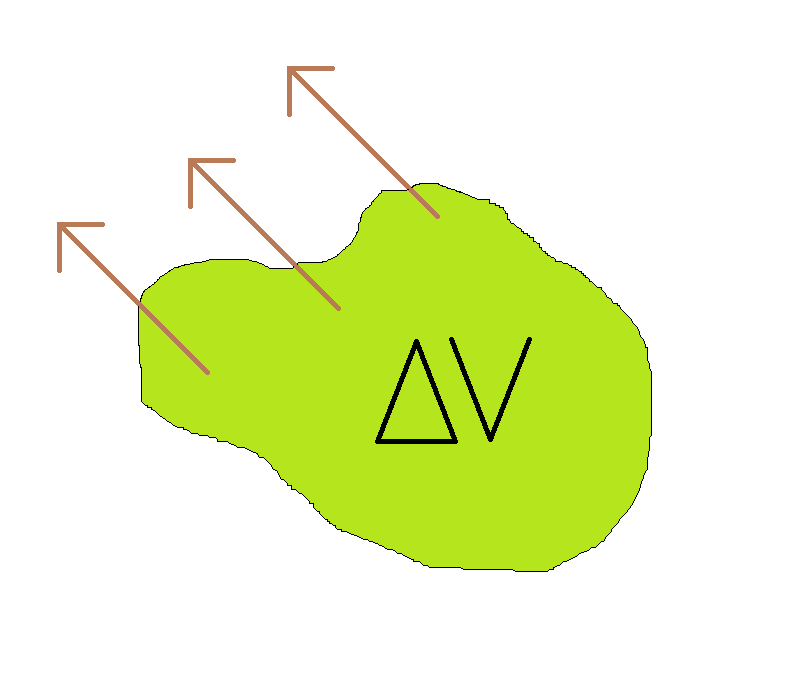
\includegraphics[height=3.5cm]{./deltaV.png} %deltaV.png
	\centering
	\caption{Kis anyagdarab, melynek minden pontja ugyanannyival megy odébb.}
	\label{fig:deltaV}
	\end{figure}
Ezt jellemzi $\rho(\underline{r},t)$, azaz sűrűsége, mely függhet helytől és időtől. Utóbbi ugye azt jelentené, hogy a vizsgált anyagdarab $\mathrm{d}t$-vel később már nem biztos, hogy ugyanabban a térfogatban helyezkedik el, s problémát okozna, hogy hova ment át. Rugalmasságtanban azonban, mivel kis deformációkat vizsgálunk (melyben a térfogatváltozás kicsi), $\rho$ időfüggésétől eltekinthetünk. (A mozgástörvényben $\rho$-t a gyorsulással kell megszorozni -ami $\underline{\ddot{u}}$-; ha felbotom $\rho$-t, mint egy alapsűrűség és a kis megváltozás, a kis megváltozást $\underline{\ddot{u}}$-vel szorozva -ahol $\underline{\ddot{u}}$ szintén pici- elhanyagolható.) Azaz $\rho(\underline{r},t)$-t tekinthetjük konstansnak. (Gázok esetén ezt nem tehetjük meg, de a víz például egész jó közelítéssel összenyomhatatlan.)
\newline
Tudjuk, hogy $\underline{v}=\frac{\partial \underline{u}}{\partial t}$. A gyorsulás esetében azonban a szubsztanciális deriváltat kéne használni, miszerint $\underline{a}=\frac{\partial \underline{v}}{\partial t}+(\underline{v} \underline{\nabla})\underline{v}$. Szerencsére mondhatjuk, hogy mivel $\underline{u}$ kicsi, és $\underline{v}$ is kicsi, így $\underline{v}\cdot\underline{v}$ már másodrendben kicsi, így elhagyható (nemúgy a hidrodinamikában). Tehát linearizálva $\underline{a}\approx\frac{\partial \underline{v}}{\partial t}\approx\frac{\partial^{2} \underline{u}}{\partial t^{2}}$, így az $m\cdot\underline{a}$ kontinuumra
	\begin{equation}
\rho\Delta V\cdot\frac{\partial^{2} \underline{u}}{\partial t^{2}}
	\label{eq:ma}
	\end{equation}
alakban adódik. %ma kontinuumra
\newline
\newline
Biztosak lehetünk abban, hogy mivel pontrendszerről van szó, a pontrendszerre vonatkozó általános tételek (Newton-axiómák) igazak maradnak. Akármekkora $\Delta V$ térfogatot is veszünk, annak a térfogatnak az össztömege megszorozva a térfogatban lévő anyag tömegközéppontjának gyorsulásával megegyezik a külső erők összegével.
\newline
Vezessük be $\underline{f^{k}}(\underline{r},t)$ erősűrűséget, mint $\frac{\Delta\underline{F^{k}}}{\Delta V}$, ahol $\Delta\underline{F^{k}}$ a kis térfogatra ható össz külső erő! Ekkor felírhatjuk, hogy a kontinuumon kívül eső erők eredője 
\[\underline{F^{k}}=\int\underline{f^{k}}(\underline{r},t)\quad\mathrm{d}V\] %Fk
\newline
Fontos megjegyezni, hogy külső erők alatt nem csak a gravitációs, elektromos, stb. terekét kell érteni /valódi külső erők/ (mint merev testek esetén), hanem a rendszer belső és külső pontjai közt fellépő erőket is (\ref{fig:belsof}.\hspace{1mm}ábra)!
	\begin{figure}[!h]
	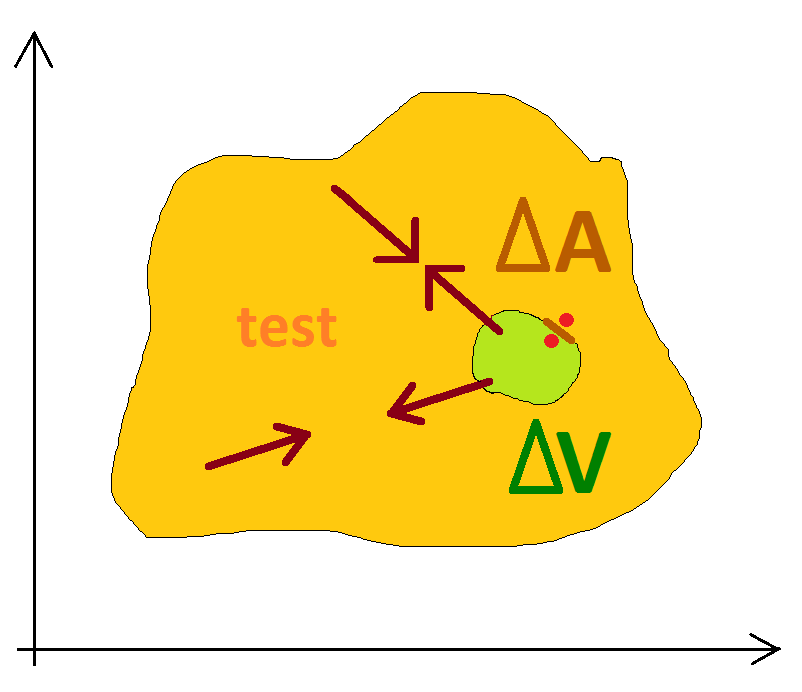
\includegraphics[height=4.5cm]{./belsof.png} %belsof.png
	\centering
	\caption{Kis anyagdarabra a rendszer rajta kívül eső pontjai is fejtenek ki erőt.}
	\label{fig:belsof}
	\end{figure}
(Ez jelentős bonyodalmat jelent például plazmafizikában, ahol a töltött részecskék vonzzák egymást, így pontonként kell felírni az összes külső erőt, ami minden pontra már egy bonyolult kettősintegrálként jelenik meg... Azonban:) \textit{Szilárd testek, illetve folyadékok esetén az atomok közt rövidtávú kölcsönhatások lépnek fel!} Ami annyit jelent, hogy a fellépő erők néhány rácsállandón belül lecsengenek (2 \si{\angstrom} körül). (Plazma esetén az $\frac{1}{r^{2}}$-tel arányos erő elég lassan csökken ahhoz, hogy ne lehessen eképp egyszerűsíteni.)
Tehát a távoli részek közt ható erők nem számítanak, csak a közvetlen szomszédok "érzik egymást", azaz a kis térfogatot határoló felület két oldalán levők (mint \aref{fig:belsof}.\hspace{1mm}ábrán a piros pöttyök). Ez alapján felírhatjuk a rugalmas erőt, mint felületi erőt $\Delta\underline{F^{r}}=\underline{P}\cdot\Delta A$, ahol $\underline{P}$ csak a felületen értelmezett mező, s így a teljes $\Delta V$-re
\[\underline{F^{r}}=\oint\underline{P}(\underline{r})\quad\mathrm{d}A\]
felszíni integrált kapjuk. %Fr
\newline
Tapasztalati tény, hogy gravitációs térben elhelyezkedő rugalmas testben ugyan a saját összenyomódásából származó rugalmas erők is szerepet játszanak -a felső rétegek nyomják az alattuk levőket-, a test tud nyugalomban lenni; létezik a rugalmas- és a gravitációs erőnek egyensúlya. (Ellentétben az elektrosztatikával, ahol két töltés nem lehet úgy nyugalomban, hogy köztük csak elektromos erők hassanak.) A fentiek alapján felírható mozgásegyenlet
	\begin{equation}
 l i m_{\Delta V\to 0} \  \rho\Delta V\cdot\frac{\partial^{2}\underline{u}}{\partial t^{2}}: \ \int_{V}\rho\underline{\ddot{u}}\quad\mathrm{d}V=\frac{\mathrm{d}\underline{p}}{\mathrm{d}t}=\underline{F_{v}}=\int_{V}\underline{f^{k}}\quad\mathrm{d}V+\oint_{\partial V}\underline{P}\quad\mathrm{d}A
	\label{eq:Fv}
	\end{equation} %Fv
(ahol $\underline{F_{v}}$ a kis $\Delta V$ alrendszerre vonatkozó eredőerő, $\underline{p}$ pedig a kis alrendszer összimpulzusa) nyugalomban nullát ad ($\frac{\partial^{2}\underline{u}}{\partial t^{2}}=0$). Azaz
	\begin{equation}
-\int\underline{f^{k}}\quad\mathrm{d}V=\oint\underline{P}\quad\mathrm{d}A
	\label{eq:gauss}
	\end{equation}
Ha ezt a jobboldali tagot átírjuk térfogati integrállá, és egyoldalra rendezünk, azt kapjuk, hogy
	\begin{equation}
\int\bigg(\underline{f^{r}}+\underline{f^{k}}\bigg)\quad\mathrm{d}V=0
	\label{eq:kiegy}
	\end{equation}
ami csak akkor lehet igaz minden térfogatra, ha a zárójelben lévő kifejezés maga nulla; azaz \textbf{a külső- és a rugalmas erők mindenhol kiegyenlítik egymást}. %kiegy
\newline
Node a Gauss-tétel (a vizsgált térfogatot körülölelő zárt felület mentén vett) felületi integrálról szól, nem felszíniről!
\[\oint\underline{v}\quad\mathrm{d}\underline{F}=\int(\underline{\nabla}\underline{v})\quad\mathrm{d}V\]
Alakítsuk hát át az alapján, hogy a felületelemvektort átírjuk $\underline{n}\mathrm{d}A$ alakba, ahol $\mathrm{d}A$ a felületelemvektor nagysága (magyarán a kis terület), $\underline{n}$ pedig a felület normálvektora.
\[\oint\bigg(\underline{v}(\underline{r})\underline{n}(\underline{r})\bigg)\quad\mathrm{d}A=\int\bigg(\underline{\nabla}\underline{v}(\underline{r})\bigg)\quad\mathrm{d}V\]
$\underline{v}(\underline{r})\underline{n}(\underline{r})$ és $\underline{\nabla}\underline{v}(\underline{r})$ definiálnak egy $\Phi(\underline{r})$, illetve $\Psi(\underline{r})$ skalármezőt:
\[\oint\Phi(\underline{r})\quad\mathrm{d}A=\int\Psi(\underline{r})\quad\mathrm{d}V\]
Azonban $\Phi(\underline{r})$, és $\Psi(\underline{r})$ nem függetlenek egymástól, létezik egy $\underline{v}$ vektormező, melyből származtathatóak. %Gauss
\newline
Ilyen alakra hozva \aref{eq:gauss}.\hspace{1mm}egyenlet jobboldalát igazolhatjuk \aref{eq:kiegy}.\hspace{1mm}összefüggés helyességét. Ehhez szorozzunk be skalárisan egy tetszőleges $\underline{c}$ vektorral! Azt kapjuk, hogy
\[\oint\underline{c}\underline{P}(\underline{r})\quad\mathrm{d}A=\int\underline{c}\underline{f^{r}}(\underline{r})\quad\mathrm{d}V\]
ahol $\underline{c}\underline{P}(\underline{r})$-t $\Phi(\underline{r})$-vel, $\underline{c}\underline{f^{r}}(\underline{r})$-t $\Psi(\underline{r})$-vel jelölve épp visszakapjuk a Gauss-tételt.
\newline
Mit tudunk $\Phi(\underline{r})$-ről és $\Psi(\underline{r})$-ről?
\newline
Az egyenlet akkor értelmes, ha $\Phi(\underline{r})$ (ami ugye $\underline{c}\underline{P}(\underline{r})$) felírható $\underline{n}(\underline{r})\underline{v}(\underline{r})$ skaláris szorzatként, ahogy $\Psi(\underline{r})$ (ami meg $\underline{c}\underline{f^{r}}(\underline{r})$) pedig $\underline{\nabla}\underline{v}(\underline{r})$-ként. Eisteini némaindexes konvencióval élve azt mondhatjuk, hogy $n_{k}v_{k}=c_{l}P_{l}$ és $\partial_{k}v_{k}=c_{l}f^{r}_{l}$. Írjuk fel $\underline{v}$-t $\underline{c}$-vel -mivel $\underline{c}$ akármilyen vektor lehet-, azaz legyen $v_{k}=c_{l}\sigma_{lk}$! Ekkor $\Phi=c_{l}\sigma_{lk}n_{k}$, és $\Psi=c_{l}\partial_{k}\sigma_{lk}$ (mert $\underline{c}$ konstansvektor, így kiemelhető a deriválás alól). S lám, megkaptuk $\underline{P}$-t, mint $\underline{\underline{\sigma}}\underline{n}$, és $\underline{f}^{r}$-t, mint $\underline{\nabla}\underline{\underline{\sigma}}$ tenzordivergencia. Ezzel bevezettük $\hat{\sigma}$ \textbf{feszültségtenzort}:
\[\Delta\underline{F^{r}}=\underline{\underline{\sigma}}\Delta\underline{F}\]
ahol $\Delta\underline{F^{r}}$ a kis felületdarabka kétoldalán lévő atomok közti kölcsönhatásból származó rugalmas erő, $\underline{\underline{\sigma}}$ a feszültségtenzor, és $\Delta\underline{F}$ a felületelemvektor.
\newline
\Aref{eq:Fv}.\hspace{1mm}egyenletet ez alapján indexesen írva:
\[F_{v_{i}}=\int(f^{k}_{i}+\frac{\partial\sigma_{ij}}{\partial r_{j}})\mathrm{d}V\] %fesztenzor
Ezt egyoldalra rendezve kapjuk
	\begin{equation}
\int_{V}\biggl[\rho\ddot{u}_{i}-f^{k}_{i}-\frac{\partial\sigma_{ij}}{\partial r_{j}}\biggr]\mathrm{d}V
	\label{eq:int} = 0
	\end{equation}
a \textbf{mozgásegyenlet integrális alakját}. S mivelhogy ennek minden $V$-re igaznak kell lennie, felírhatjuk \textbf{differenciális alakban} is:
	\begin{equation}
\rho\underline{\ddot{u}}=\underline{f^{k}}+\underline{\nabla}\underline{\underline{\sigma}}
	\label{eq:diff}
	\end{equation}
\newline
\newline
Node! Nem elég az egyensúlyhoz, hogy az erők eredője nulla legyen, a forgatónyomatékoknak is nulla eredőt kell adniuk. A kis $\Delta V$-re felírva a forgatónyomatékot (jelöléseket lásd \aref{fig:M}.\hspace{1mm}ábrán)
	\begin{figure}[!h]
	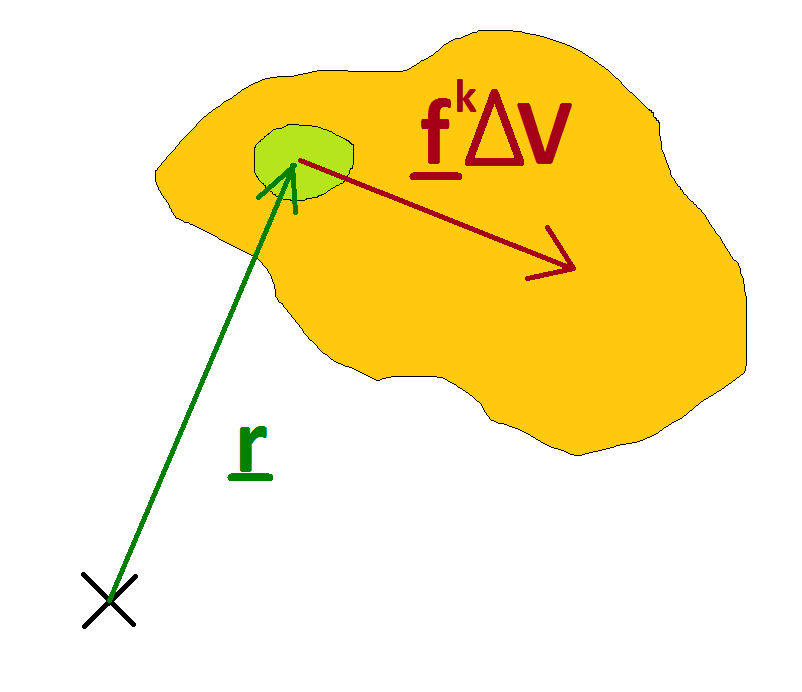
\includegraphics[height=3.5cm]{./M.png} %M.png
	\centering
	\caption{Kis anyagdarabra ható forgatónyomaték.}
	\label{fig:M}
	\end{figure}
adódik
\[\Delta\underline{M^{k}}=\underline{r}\times\Delta\underline{F^{k}}=\underline{r}\times\underline{f^{k}}\Delta V\]
és
\[\Delta\underline{M^{r}}=\underline{r}\times\Delta\underline{F^{r}}=\underline{r}\times\underline{P}\Delta A\]
egyenletekből
	\begin{equation}
\underline{M}=\int\underline{r}\times\underline{f^{k}}\quad\mathrm{d}V+\oint\underline{r}\times\underline{P}\quad\mathrm{d}A\equiv 0
	\label{eq:M}
	\end{equation}
ahol tudjuk, hogy $\underline{f^{k}}=-\underline{f^{r}}$, $\underline{f^{r}}$ pedig $\underline{\nabla}\underline{\underline{\sigma}}$ és $\underline{P}=\underline{\underline{\sigma}}\underline{n}$. \Aref{eq:M}.\hspace{1mm}egyenletbe ezeket behelyettesítve és indexesen rendezve:
\[M_{k}=\int\mathrm{d}V\quad\varepsilon_{klm}r_{l}f^{k}_{m}+\oint\mathrm{d}A\quad\varepsilon_{klm}r_{l}P_{m}\]
\[=\int\mathrm{d}V\quad\varepsilon_{klm}r_{l}(-f^{r}_{m})+\oint\mathrm{d}A\quad\varepsilon_{klm}r_{l}P_{m}\]
\[=-\int\mathrm{d}V\quad\varepsilon_{klm}r_{l}\partial_{s}\sigma_{ms}+\oint\mathrm{d}A\quad\varepsilon_{klm}r_{l}\sigma_{ms}n_{s}\]
$\mathrm{d}A\cdot n_{s}$ viszont $\mathrm{d}F_{s}$, így kiemelve $\varepsilon_{klm}$-t, s Gauss-tétel alapján tovább alakítva:
\[M_{k}=\varepsilon_{klm}\Bigg(-\int\mathrm{d}V\quad r_{l}\partial_{s}\sigma_{ms}+\oint\mathrm{d}F_{s}\quad r_{l}\sigma_{ms}\Bigg)\]
\[=\varepsilon_{klm}\int\mathrm{d}V\bigg(\partial_{s}(r_{l}\sigma_{ms})-r_{l}\partial_{s}\sigma_{ms}\bigg)\]
Végezzük el a deriválást!
\[M_{k}=\varepsilon_{klm}\int\mathrm{d}V\bigg((\partial_{s}r_{l})\sigma_{ms}+r_{l}\partial_{s}\sigma_{ms}-r_{l}\partial_{s}\sigma_{ms}\bigg)\]
Nagyon örülünk, mert az utolsó két tag kiejti egymást, $\partial_{s}r_{l}$ pedig $\delta_{sl}$, a Kronecker-delta pedig beírja $l$-t $s$ helyére $\sigma$-ban:
\[M_{k}=\varepsilon_{klm}\int\mathrm{d}V\quad\sigma_{ml}\]
$\varepsilon_{klm}$-et visszavíve az integrál alá kapjuk, hogy
\[\int\mathrm{d}V(\varepsilon_{klm}\sigma_{ml})=M_{k}\equiv 0\]
Megfigyelve az indexeket (mivel a Levi-Civita szimbólum antiszimmetrikus) ez a mennyiség csak akkor lehet nulla, ha \textbf{a feszültségtenzor szimmetrikus}! Tehát
	\begin{equation}
\sigma_{ij}=\sigma_{ji}
	\label{eq:szimm}
	\end{equation}
Ez elegendő feltétel ahhoz, hogy a forgatónyomaték is nulla legyen minden tengelyre, $\frac{\mathrm{d}\underline{N}}{\mathrm{d}t}=\underline{M}$. (Ha $\hat{\sigma}$ szimmetrikussága nem teljesül, be kell vezetni a forgatónyomatéksűrűséget.)
\newline
Már csak azt kell megvizsgálnunk, mitől függhet a feszültségtenzor. Szilárd anyag esetén $\hat{\varepsilon}$ deformációs tenzoron keresztül függ $\underline{u}$-tól és helyszerinti deriváltjaitól. Folyadékok esetén $\hat{\varepsilon}$ első deriváltjától függ csupán, de léteznek összetett anyagok (például kátrány, gyurmalin -avagy inteligens gyurma-), melynél $\sigma(\hat{\varepsilon},\dot{\hat{\varepsilon}})$.



%\SI{1}{\angstrom} vagy \si{\angstrom}




\end{document}
